\documentclass{article}

\usepackage{graphicx}
\usepackage{tikz}
\usepackage{tikzsymbols}
\usetikzlibrary{calc,patterns,shapes.geometric}
\pagestyle{empty}
\usepackage[margin=0pt]{geometry}
\geometry{papersize={14in,12in}}

\def\centerarc[#1](#2)(#3:#4:#5){\draw[#1] ($(#2)+({#5*cos(#3)},{#5*sin(#3)})$) arc (#3:#4:#5);}

\begin{document}
	\begin{figure}
		\centering
		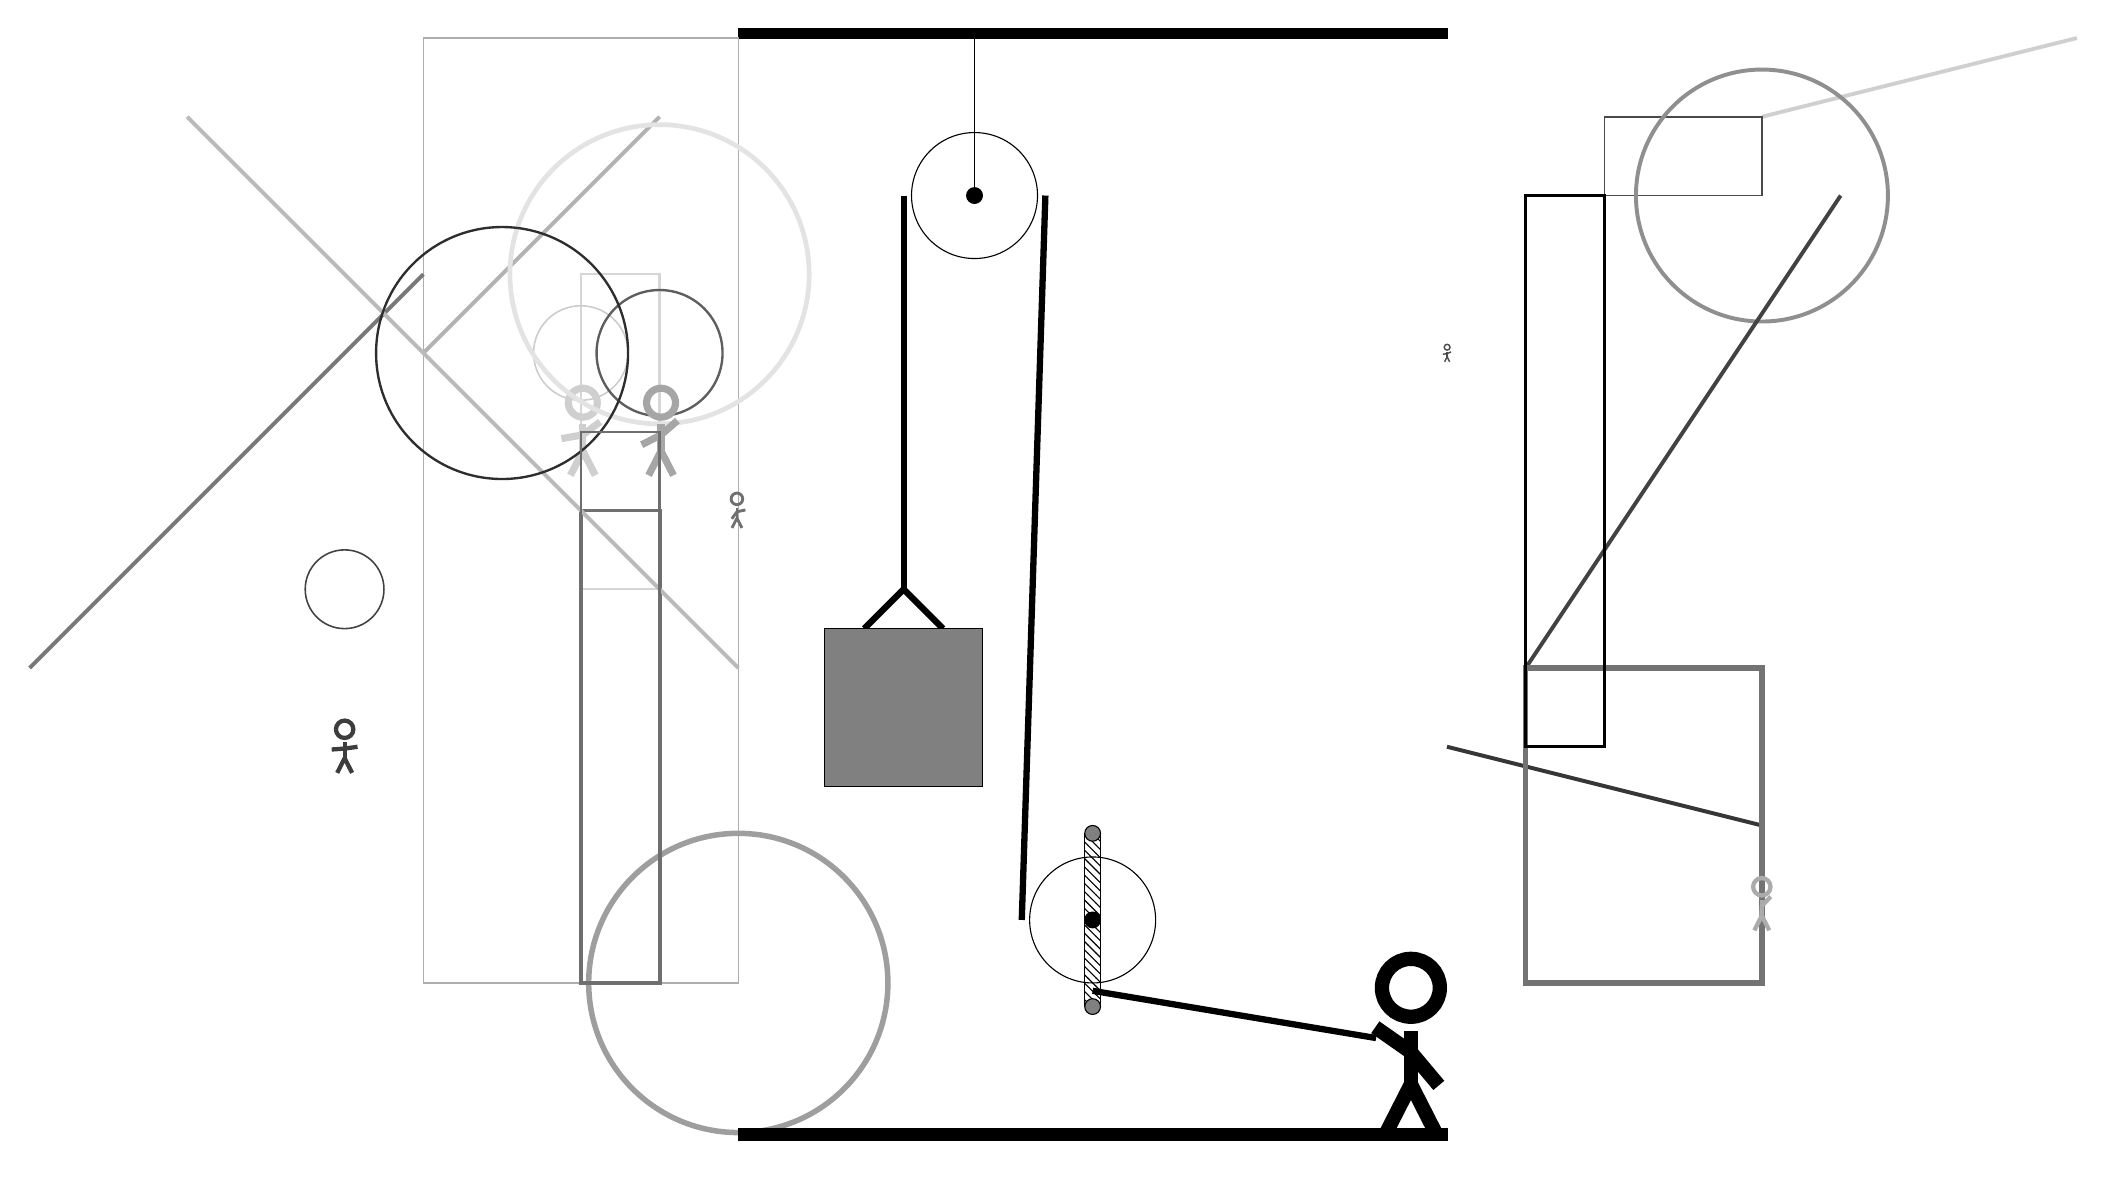
\begin{tikzpicture}
			%%%%% START %%%%%
			
			\draw[fill=black] (-2, 14) rectangle (7, 14.125);
			
			\draw (1, 12) circle (0.8);
			\draw[fill=black] (1, 12) circle (0.1);
			\draw (1, 14) -- (1, 12);
			
			\draw[line width=0.3mm, color=black!16] (-3, 11) rectangle (-4, 7);
			
			\draw[line width=0.5mm, color=black!19](11, 13) -- (15, 14);
			\draw[line width=0.2mm, color=black!71] (9, 13) rectangle (11, 12);
			\draw [line width=0.2mm, color=black!20](-4, 10) circle (0.6);
			
			\draw[line width=0.2mm, color=black!32] (-2, 2) rectangle (-6, 14);
			\draw [line width=0.5mm, color=black!44](11, 12) circle (1.6);
			\node[line width=0.2mm, color=black!70] at (7, 10) {\Strichmaxerl[1][8][24]};
			
			\node[line width=0.6mm, color=black!56] at (-2, 8) {\Strichmaxerl[2][54][12]};
			\node[line width=0.5mm, color=black!19] at (-4, 9) {\Strichmaxerl[5][10][37]};
			\draw[line width=0.5mm, color=black!30](-6, 10) -- (-3, 13);
			\draw [line width=0.3mm, color=black!63](-3, 10) circle (0.8);
			
			\draw [line width=0.7mm, color=black!38](-2, 2) circle (1.9);
			\draw[line width=0.5mm, color=black!74](12, 12) -- (8, 6);
			
			\draw[line width=0.5mm, color=black!79](7, 5) -- (11, 4);
			\draw [line width=0.2mm, color=black!74](-7, 7) circle (0.5);
			\node[line width=0.6mm, color=black!76] at (-7, 5) {\Strichmaxerl[3][4][8]};
			
			\draw[line width=0.7mm, color=black!55] (8, 6) rectangle (11, 2);
			\draw[line width=0.5mm, color=black!53](-6, 11) -- (-11, 6);
			\node[line width=0.3mm, color=black!33] at (11, 3) {\Strichmaxerl[3][88][47]};
			\draw[line width=0.5mm, color=black!56] (-3, 8) rectangle (-4, 2);
			\draw[line width=0.4mm, color=black!100] (8, 12) rectangle (9, 5);
			\draw[line width=0.5mm, color=black!27](-2, 6) -- (-9, 13);
			
			\draw [line width=0.6mm, color=black!11](-3, 11) circle (1.9);
			\draw [line width=0.3mm, color=black!82](-5, 10) circle (1.6);
			\node[line width=0.2mm, color=black!35] at (-3, 9) {\Strichmaxerl[5][27][41]};
			
			\draw[line width=0.3mm, color=black!57] (-3, 2) rectangle (-4, 9);
			
			
			\draw[fill=white](2.5, 2.8) circle (0.8);
			\draw[fill=black] (2.5, 2.8) circle (0.1);
			\draw[pattern=north west lines, pattern color=black] (2.4, 3.9) rectangle (2.6, 1.7);
			\draw[fill=black!50] (2.5, 3.9) circle (0.1);
			\draw[fill=black!50] (2.5, 1.7) circle (0.1);
			
			\draw[line width=0.8mm] (-0.4, 6.5) -- (0.1, 7.0) -- (0.6, 6.5);
			\draw[fill=black!50] (-0.9, 6.5) rectangle (1.1, 4.5);
			
			\draw[line width=0.8mm] (0.1, 12) -- (0.1, 7.0);
			\centerarc[line width=0.8mm](1, 12)(0:180:0.9);
			\draw[line width=0.8mm](1.9, 12) -- (1.6, 2.8);
			\centerarc[line width=0.8mm](2.5, 2.8)(180:270:0.9);
			\draw[line width=0.8mm](2.5, 1.9) -- (6.1, 1.3);
			
			\node at (6.5, 1.2) {\Strichmaxerl[10][-35][-50]};
			
			\draw[fill=black] (-2, 0) rectangle (7, 0.15);
			
			%%%%% END %%%%%
		\end{tikzpicture}
	\end{figure}	
\end{document}